% Options for packages loaded elsewhere
\PassOptionsToPackage{unicode}{hyperref}
\PassOptionsToPackage{hyphens}{url}
%
\documentclass[
]{book}
\usepackage{amsmath,amssymb}
\usepackage{iftex}
\ifPDFTeX
  \usepackage[T1]{fontenc}
  \usepackage[utf8]{inputenc}
  \usepackage{textcomp} % provide euro and other symbols
\else % if luatex or xetex
  \usepackage{unicode-math} % this also loads fontspec
  \defaultfontfeatures{Scale=MatchLowercase}
  \defaultfontfeatures[\rmfamily]{Ligatures=TeX,Scale=1}
\fi
\usepackage{lmodern}
\ifPDFTeX\else
  % xetex/luatex font selection
\fi
% Use upquote if available, for straight quotes in verbatim environments
\IfFileExists{upquote.sty}{\usepackage{upquote}}{}
\IfFileExists{microtype.sty}{% use microtype if available
  \usepackage[]{microtype}
  \UseMicrotypeSet[protrusion]{basicmath} % disable protrusion for tt fonts
}{}
\makeatletter
\@ifundefined{KOMAClassName}{% if non-KOMA class
  \IfFileExists{parskip.sty}{%
    \usepackage{parskip}
  }{% else
    \setlength{\parindent}{0pt}
    \setlength{\parskip}{6pt plus 2pt minus 1pt}}
}{% if KOMA class
  \KOMAoptions{parskip=half}}
\makeatother
\usepackage{xcolor}
\usepackage{color}
\usepackage{fancyvrb}
\newcommand{\VerbBar}{|}
\newcommand{\VERB}{\Verb[commandchars=\\\{\}]}
\DefineVerbatimEnvironment{Highlighting}{Verbatim}{commandchars=\\\{\}}
% Add ',fontsize=\small' for more characters per line
\usepackage{framed}
\definecolor{shadecolor}{RGB}{248,248,248}
\newenvironment{Shaded}{\begin{snugshade}}{\end{snugshade}}
\newcommand{\AlertTok}[1]{\textcolor[rgb]{0.94,0.16,0.16}{#1}}
\newcommand{\AnnotationTok}[1]{\textcolor[rgb]{0.56,0.35,0.01}{\textbf{\textit{#1}}}}
\newcommand{\AttributeTok}[1]{\textcolor[rgb]{0.13,0.29,0.53}{#1}}
\newcommand{\BaseNTok}[1]{\textcolor[rgb]{0.00,0.00,0.81}{#1}}
\newcommand{\BuiltInTok}[1]{#1}
\newcommand{\CharTok}[1]{\textcolor[rgb]{0.31,0.60,0.02}{#1}}
\newcommand{\CommentTok}[1]{\textcolor[rgb]{0.56,0.35,0.01}{\textit{#1}}}
\newcommand{\CommentVarTok}[1]{\textcolor[rgb]{0.56,0.35,0.01}{\textbf{\textit{#1}}}}
\newcommand{\ConstantTok}[1]{\textcolor[rgb]{0.56,0.35,0.01}{#1}}
\newcommand{\ControlFlowTok}[1]{\textcolor[rgb]{0.13,0.29,0.53}{\textbf{#1}}}
\newcommand{\DataTypeTok}[1]{\textcolor[rgb]{0.13,0.29,0.53}{#1}}
\newcommand{\DecValTok}[1]{\textcolor[rgb]{0.00,0.00,0.81}{#1}}
\newcommand{\DocumentationTok}[1]{\textcolor[rgb]{0.56,0.35,0.01}{\textbf{\textit{#1}}}}
\newcommand{\ErrorTok}[1]{\textcolor[rgb]{0.64,0.00,0.00}{\textbf{#1}}}
\newcommand{\ExtensionTok}[1]{#1}
\newcommand{\FloatTok}[1]{\textcolor[rgb]{0.00,0.00,0.81}{#1}}
\newcommand{\FunctionTok}[1]{\textcolor[rgb]{0.13,0.29,0.53}{\textbf{#1}}}
\newcommand{\ImportTok}[1]{#1}
\newcommand{\InformationTok}[1]{\textcolor[rgb]{0.56,0.35,0.01}{\textbf{\textit{#1}}}}
\newcommand{\KeywordTok}[1]{\textcolor[rgb]{0.13,0.29,0.53}{\textbf{#1}}}
\newcommand{\NormalTok}[1]{#1}
\newcommand{\OperatorTok}[1]{\textcolor[rgb]{0.81,0.36,0.00}{\textbf{#1}}}
\newcommand{\OtherTok}[1]{\textcolor[rgb]{0.56,0.35,0.01}{#1}}
\newcommand{\PreprocessorTok}[1]{\textcolor[rgb]{0.56,0.35,0.01}{\textit{#1}}}
\newcommand{\RegionMarkerTok}[1]{#1}
\newcommand{\SpecialCharTok}[1]{\textcolor[rgb]{0.81,0.36,0.00}{\textbf{#1}}}
\newcommand{\SpecialStringTok}[1]{\textcolor[rgb]{0.31,0.60,0.02}{#1}}
\newcommand{\StringTok}[1]{\textcolor[rgb]{0.31,0.60,0.02}{#1}}
\newcommand{\VariableTok}[1]{\textcolor[rgb]{0.00,0.00,0.00}{#1}}
\newcommand{\VerbatimStringTok}[1]{\textcolor[rgb]{0.31,0.60,0.02}{#1}}
\newcommand{\WarningTok}[1]{\textcolor[rgb]{0.56,0.35,0.01}{\textbf{\textit{#1}}}}
\usepackage{longtable,booktabs,array}
\usepackage{calc} % for calculating minipage widths
% Correct order of tables after \paragraph or \subparagraph
\usepackage{etoolbox}
\makeatletter
\patchcmd\longtable{\par}{\if@noskipsec\mbox{}\fi\par}{}{}
\makeatother
% Allow footnotes in longtable head/foot
\IfFileExists{footnotehyper.sty}{\usepackage{footnotehyper}}{\usepackage{footnote}}
\makesavenoteenv{longtable}
\usepackage{graphicx}
\makeatletter
\newsavebox\pandoc@box
\newcommand*\pandocbounded[1]{% scales image to fit in text height/width
  \sbox\pandoc@box{#1}%
  \Gscale@div\@tempa{\textheight}{\dimexpr\ht\pandoc@box+\dp\pandoc@box\relax}%
  \Gscale@div\@tempb{\linewidth}{\wd\pandoc@box}%
  \ifdim\@tempb\p@<\@tempa\p@\let\@tempa\@tempb\fi% select the smaller of both
  \ifdim\@tempa\p@<\p@\scalebox{\@tempa}{\usebox\pandoc@box}%
  \else\usebox{\pandoc@box}%
  \fi%
}
% Set default figure placement to htbp
\def\fps@figure{htbp}
\makeatother
\setlength{\emergencystretch}{3em} % prevent overfull lines
\providecommand{\tightlist}{%
  \setlength{\itemsep}{0pt}\setlength{\parskip}{0pt}}
\setcounter{secnumdepth}{5}
\usepackage{booktabs}
\usepackage[]{natbib}
\bibliographystyle{apalike}
\usepackage{bookmark}
\IfFileExists{xurl.sty}{\usepackage{xurl}}{} % add URL line breaks if available
\urlstyle{same}
\hypersetup{
  pdftitle={The Jungle},
  pdfauthor={Upton Sinclair},
  hidelinks,
  pdfcreator={LaTeX via pandoc}}

\title{The Jungle}
\author{Upton Sinclair}
\date{2025-06-10}

\usepackage{amsthm}
\newtheorem{theorem}{Theorem}[chapter]
\newtheorem{lemma}{Lemma}[chapter]
\newtheorem{corollary}{Corollary}[chapter]
\newtheorem{proposition}{Proposition}[chapter]
\newtheorem{conjecture}{Conjecture}[chapter]
\theoremstyle{definition}
\newtheorem{definition}{Definition}[chapter]
\theoremstyle{definition}
\newtheorem{example}{Example}[chapter]
\theoremstyle{definition}
\newtheorem{exercise}{Exercise}[chapter]
\theoremstyle{definition}
\newtheorem{hypothesis}{Hypothesis}[chapter]
\theoremstyle{remark}
\newtheorem*{remark}{Remark}
\newtheorem*{solution}{Solution}
\begin{document}
\maketitle

{
\setcounter{tocdepth}{1}
\tableofcontents
}
\chapter{\texorpdfstring{\href{https://www.marxists.org/history/usa/pubs/appeal-to-reason/050225-appealtoreason-w482-thejungle.pdf}{A Packingtown Wedding}}{A Packingtown Wedding}}\label{a-packingtown-wedding}

It was four o'clock when the ceremony was over and the carriages began to arrive. There had been a crowd following all the way, owing to the exuberance of Marija Berczynskas. The occasion rested heavily upon Marija's broad shoulders---it was her task to see that all things went in due form, and after the best home traditions; and, flying wildly hither and thither, bowling every one out of the way, and scolding and exhorting all day with her tremendous voice, Marija was too eager to see that others conformed to the proprieties to consider them herself. She had left the church last of all, and, desiring to arrive first at the hall, had issued orders to the coachman to drive faster. When that personage had developed a will of his own in the matter, Marija had flung up the window of the carriage, and, leaning out, proceeded to tell him her opinion of him, first in Lithuanian, which he did not understand, and then in Polish, which he did. Having the advantage of her in altitude, the driver had stood his ground and even ventured to attempt to speak; and the result had been a furious altercation, which, continuing all the way down Ashland Avenue, had added a new swarm of urchins to the cortege at each side street for half a mile.

This was unfortunate, for already there was a throng before the door. The music had started up, and half a block away you could hear the dull ``broom, broom'' of a cello, with the squeaking of two fiddles which vied with each other in intricate and altitudinous gymnastics. Seeing the throng, Marija abandoned precipitately the debate concerning the ancestors of her coachman, and, springing from the moving carriage, plunged in and proceeded to clear a way to the hall. Once within, she turned and began to push the other way, roaring, meantime, ``Eik! Eik! Uzdaryk-duris!'' in tones which made the orchestral uproar sound like fairy music.

``Z. Graiczunas, Pasilinksminimams darzas. Vynas. Sznapsas. Wines and Liquors. Union Headquarters''---that was the way the signs ran. The reader, who perhaps has never held much converse in the language of far-off Lithuania, will be glad of the explanation that the place was the rear room of a saloon in that part of Chicago known as ``back of the yards.'' This information is definite and suited to the matter of fact; but how pitifully inadequate it would have seemed to one who understood that it was also the supreme hour of ecstasy in the life of one of God's gentlest creatures, the scene of the wedding feast and the joy-transfiguration of little Ona Lukoszaite!

She stood in the doorway, shepherded by Cousin Marija, breathless from pushing through the crowd, and in her happiness painful to look upon. There was a light of wonder in her eyes and her lids trembled, and her otherwise wan little face was flushed. She wore a muslin dress, conspicuously white, and a stiff little veil coming to her shoulders. There were five pink paper roses twisted in the veil, and eleven bright green rose leaves. There were new white cotton gloves upon her hands, and as she stood staring about her she twisted them together feverishly. It was almost too much for her---you could see the pain of too great emotion in her face, and all the tremor of her form. She was so young---not quite sixteen---and small for her age, a mere child; and she had just been married---and married to Jurgis,{[}1{]} of all men, to Jurgis Rudkus, he with the white flower in the buttonhole of his new black suit, he with the mighty shoulders and the giant hands.

Ona was blue-eyed and fair, while Jurgis had great black eyes with beetling brows, and thick black hair that curled in waves about his ears---in short, they were one of those incongruous and impossible married couples with which Mother Nature so often wills to confound all prophets, before and after. Jurgis could take up a two-hundred-and-fifty-pound quarter of beef and carry it into a car without a stagger, or even a thought; and now he stood in a far corner, frightened as a hunted animal, and obliged to moisten his lips with his tongue each time before he could answer the congratulations of his friends.

Gradually there was effected a separation between the spectators and the guests---a separation at least sufficiently complete for working purposes. There was no time during the festivities which ensued when there were not groups of onlookers in the doorways and the corners; and if any one of these onlookers came sufficiently close, or looked sufficiently hungry, a chair was offered him, and he was invited to the feast. It was one of the laws of the veselija that no one goes hungry; and, while a rule made in the forests of Lithuania is hard to apply in the stockyards district of Chicago, with its quarter of a million inhabitants, still they did their best, and the children who ran in from the street, and even the dogs, went out again happier. A charming informality was one of the characteristics of this celebration. The men wore their hats, or, if they wished, they took them off, and their coats with them; they ate when and where they pleased, and moved as often as they pleased. There were to be speeches and singing, but no one had to listen who did not care to; if he wished, meantime, to speak or sing himself, he was perfectly free. The resulting medley of sound distracted no one, save possibly alone the babies, of which there were present a number equal to the total possessed by all the guests invited. There was no other place for the babies to be, and so part of the preparations for the evening consisted of a collection of cribs and carriages in one corner. In these the babies slept, three or four together, or wakened together, as the case might be. Those who were still older, and could reach the tables, marched about munching contentedly at meat bones and bologna sausages.

The room is about thirty feet square, with whitewashed walls, bare save for a calendar, a picture of a race horse, and a family tree in a gilded frame. To the right there is a door from the saloon, with a few loafers in the doorway, and in the corner beyond it a bar, with a presiding genius clad in soiled white, with waxed black mustaches and a carefully oiled curl plastered against one side of his forehead. In the opposite corner are two tables, filling a third of the room and laden with dishes and cold viands, which a few of the hungrier guests are already munching. At the head, where sits the bride, is a snow-white cake, with an Eiffel tower of constructed decoration, with sugar roses and two angels upon it, and a generous sprinkling of pink and green and yellow candies. Beyond opens a door into the kitchen, where there is a glimpse to be had of a range with much steam ascending from it, and many women, old and young, rushing hither and thither. In the corner to the left are the three musicians, upon a little platform, toiling heroically to make some impression upon the hubbub; also the babies, similarly occupied, and an open window whence the populace imbibes the sights and sounds and odors.

Suddenly some of the steam begins to advance, and, peering through it, you discern Aunt Elizabeth, Ona's stepmother---Teta Elzbieta, as they call her---bearing aloft a great platter of stewed duck. Behind her is Kotrina, making her way cautiously, staggering beneath a similar burden; and half a minute later there appears old Grandmother Majauszkiene, with a big yellow bowl of smoking potatoes, nearly as big as herself. So, bit by bit, the feast takes form---there is a ham and a dish of sauerkraut, boiled rice, macaroni, bologna sausages, great piles of penny buns, bowls of milk, and foaming pitchers of beer. There is also, not six feet from your back, the bar, where you may order all you please and do not have to pay for it. ``Eiksz! Graicziau!'' screams Marija Berczynskas, and falls to work herself---for there is more upon the stove inside that will be spoiled if it be not eaten.

So, with laughter and shouts and endless badinage and merriment, the guests take their places. The young men, who for the most part have been huddled near the door, summon their resolution and advance; and the shrinking Jurgis is poked and scolded by the old folks until he consents to seat himself at the right hand of the bride. The two bridesmaids, whose insignia of office are paper wreaths, come next, and after them the rest of the guests, old and young, boys and girls. The spirit of the occasion takes hold of the stately bartender, who condescends to a plate of stewed duck; even the fat policeman---whose duty it will be, later in the evening, to break up the fights---draws up a chair to the foot of the table. And the children shout and the babies yell, and every one laughs and sings and chatters---while above all the deafening clamor Cousin Marija shouts orders to the musicians.

The musicians---how shall one begin to describe them? All this time they have been there, playing in a mad frenzy---all of this scene must be read, or said, or sung, to music. It is the music which makes it what it is; it is the music which changes the place from the rear room of a saloon in back of the yards to a fairy place, a wonderland, a little corner of the high mansions of the sky.

The little person who leads this trio is an inspired man. His fiddle is out of tune, and there is no rosin on his bow, but still he is an inspired man---the hands of the muses have been laid upon him. He plays like one possessed by a demon, by a whole horde of demons. You can feel them in the air round about him, capering frenetically; with their invisible feet they set the pace, and the hair of the leader of the orchestra rises on end, and his eyeballs start from their sockets, as he toils to keep up with them.

Tamoszius Kuszleika is his name, and he has taught himself to play the violin by practicing all night, after working all day on the ``killing beds.'' He is in his shirt sleeves, with a vest figured with faded gold horseshoes, and a pink-striped shirt, suggestive of peppermint candy. A pair of military trousers, light blue with a yellow stripe, serve to give that suggestion of authority proper to the leader of a band. He is only about five feet high, but even so these trousers are about eight inches short of the ground. You wonder where he can have gotten them or rather you would wonder, if the excitement of being in his presence left you time to think of such things.

For he is an inspired man. Every inch of him is inspired---you might almost say inspired separately. He stamps with his feet, he tosses his head, he sways and swings to and fro; he has a wizened-up little face, irresistibly comical; and, when he executes a turn or a flourish, his brows knit and his lips work and his eyelids wink---the very ends of his necktie bristle out. And every now and then he turns upon his companions, nodding, signaling, beckoning frantically---with every inch of him appealing, imploring, in behalf of the muses and their call.

For they are hardly worthy of Tamoszius, the other two members of the orchestra. The second violin is a Slovak, a tall, gaunt man with black-rimmed spectacles and the mute and patient look of an overdriven mule; he responds to the whip but feebly, and then always falls back into his old rut. The third man is very fat, with a round, red, sentimental nose, and he plays with his eyes turned up to the sky and a look of infinite yearning. He is playing a bass part upon his cello, and so the excitement is nothing to him; no matter what happens in the treble, it is his task to saw out one long-drawn and lugubrious note after another, from four o'clock in the afternoon until nearly the same hour next morning, for his third of the total income of one dollar per hour.

Before the feast has been five minutes under way, Tamoszius Kuszleika has risen in his excitement; a minute or two more and you see that he is beginning to edge over toward the tables. His nostrils are dilated and his breath comes fast---his demons are driving him. He nods and shakes his head at his companions, jerking at them with his violin, until at last the long form of the second violinist also rises up. In the end all three of them begin advancing, step by step, upon the banqueters, Valentinavyczia, the cellist, bumping along with his instrument between notes. Finally all three are gathered at the foot of the tables, and there Tamoszius mounts upon a stool.

Now he is in his glory, dominating the scene. Some of the people are eating, some are laughing and talking---but you will make a great mistake if you think there is one of them who does not hear him. His notes are never true, and his fiddle buzzes on the low ones and squeaks and scratches on the high; but these things they heed no more than they heed the dirt and noise and squalor about them---it is out of this material that they have to build their lives, with it that they have to utter their souls. And this is their utterance; merry and boisterous, or mournful and wailing, or passionate and rebellious, this music is their music, music of home. It stretches out its arms to them, they have only to give themselves up. Chicago and its saloons and its slums fade away---there are green meadows and sunlit rivers, mighty forests and snow-clad hills. They behold home landscapes and childhood scenes returning; old loves and friendships begin to waken, old joys and griefs to laugh and weep. Some fall back and close their eyes, some beat upon the table. Now and then one leaps up with a cry and calls for this song or that; and then the fire leaps brighter in Tamoszius' eyes, and he flings up his fiddle and shouts to his companions, and away they go in mad career. The company takes up the choruses, and men and women cry out like all possessed; some leap to their feet and stamp upon the floor, lifting their glasses and pledging each other. Before long it occurs to some one to demand an old wedding song, which celebrates the beauty of the bride and the joys of love. In the excitement of this masterpiece Tamoszius Kuszleika begins to edge in between the tables, making his way toward the head, where sits the bride. There is not a foot of space between the chairs of the guests, and Tamoszius is so short that he pokes them with his bow whenever he reaches over for the low notes; but still he presses in, and insists relentlessly that his companions must follow. During their progress, needless to say, the sounds of the cello are pretty well extinguished; but at last the three are at the head, and Tamoszius takes his station at the right hand of the bride and begins to pour out his soul in melting strains.

Little Ona is too excited to eat. Once in a while she tastes a little something, when Cousin Marija pinches her elbow and reminds her; but, for the most part, she sits gazing with the same fearful eyes of wonder. Teta Elzbieta is all in a flutter, like a hummingbird; her sisters, too, keep running up behind her, whispering, breathless. But Ona seems scarcely to hear them---the music keeps calling, and the far-off look comes back, and she sits with her hands pressed together over her heart. Then the tears begin to come into her eyes; and as she is ashamed to wipe them away, and ashamed to let them run down her cheeks, she turns and shakes her head a little, and then flushes red when she sees that Jurgis is watching her. When in the end Tamoszius Kuszleika has reached her side, and is waving his magic wand above her, Ona's cheeks are scarlet, and she looks as if she would have to get up and run away.

In this crisis, however, she is saved by Marija Berczynskas, whom the muses suddenly visit. Marija is fond of a song, a song of lovers' parting; she wishes to hear it, and, as the musicians do not know it, she has risen, and is proceeding to teach them. Marija is short, but powerful in build. She works in a canning factory, and all day long she handles cans of beef that weigh fourteen pounds. She has a broad Slavic face, with prominent red cheeks. When she opens her mouth, it is tragical, but you cannot help thinking of a horse. She wears a blue flannel shirt-waist, which is now rolled up at the sleeves, disclosing her brawny arms; she has a carving fork in her hand, with which she pounds on the table to mark the time. As she roars her song, in a voice of which it is enough to say that it leaves no portion of the room vacant, the three musicians follow her, laboriously and note by note, but averaging one note behind; thus they toil through stanza after stanza of a lovesick swain's lamentation:---

\begin{quote}
``Sudiev' kvietkeli, tu brangiausis;
Sudiev' ir laime, man biednam,
Matau---paskyre teip Aukszcziausis,
Jog vargt ant svieto reik vienam!''
When the song is over, it is time for the speech, and old Dede Antanas rises to his feet. Grandfather Anthony, Jurgis' father, is not more than sixty years of age, but you would think that he was eighty. He has been only six months in America, and the change has not done him good. In his manhood he worked in a cotton mill, but then a coughing fell upon him, and he had to leave; out in the country the trouble disappeared, but he has been working in the pickle rooms at Durham's, and the breathing of the cold, damp air all day has brought it back. Now as he rises he is seized with a coughing fit, and holds himself by his chair and turns away his wan and battered face until it passes.
\end{quote}

Generally it is the custom for the speech at a veselija to be taken out of one of the books and learned by heart; but in his youthful days Dede Antanas used to be a scholar, and really make up all the love letters of his friends. Now it is understood that he has composed an original speech of congratulation and benediction, and this is one of the events of the day. Even the boys, who are romping about the room, draw near and listen, and some of the women sob and wipe their aprons in their eyes. It is very solemn, for Antanas Rudkus has become possessed of the idea that he has not much longer to stay with his children. His speech leaves them all so tearful that one of the guests, Jokubas Szedvilas, who keeps a delicatessen store on Halsted Street, and is fat and hearty, is moved to rise and say that things may not be as bad as that, and then to go on and make a little speech of his own, in which he showers congratulations and prophecies of happiness upon the bride and groom, proceeding to particulars which greatly delight the young men, but which cause Ona to blush more furiously than ever. Jokubas possesses what his wife complacently describes as ``poetiszka vaidintuve''---a poetical imagination.

Now a good many of the guests have finished, and, since there is no pretense of ceremony, the banquet begins to break up. Some of the men gather about the bar; some wander about, laughing and singing; here and there will be a little group, chanting merrily, and in sublime indifference to the others and to the orchestra as well. Everybody is more or less restless---one would guess that something is on their minds. And so it proves. The last tardy diners are scarcely given time to finish, before the tables and the debris are shoved into the corner, and the chairs and the babies piled out of the way, and the real celebration of the evening begins. Then Tamoszius Kuszleika, after replenishing himself with a pot of beer, returns to his platform, and, standing up, reviews the scene; he taps authoritatively upon the side of his violin, then tucks it carefully under his chin, then waves his bow in an elaborate flourish, and finally smites the sounding strings and closes his eyes, and floats away in spirit upon the wings of a dreamy waltz. His companion follows, but with his eyes open, watching where he treads, so to speak; and finally Valentinavyczia, after waiting for a little and beating with his foot to get the time, casts up his eyes to the ceiling and begins to saw---``Broom! broom! broom!''

The company pairs off quickly, and the whole room is soon in motion. Apparently nobody knows how to waltz, but that is nothing of any consequence---there is music, and they dance, each as he pleases, just as before they sang. Most of them prefer the ``two-step,'' especially the young, with whom it is the fashion. The older people have dances from home, strange and complicated steps which they execute with grave solemnity. Some do not dance anything at all, but simply hold each other's hands and allow the undisciplined joy of motion to express itself with their feet. Among these are Jokubas Szedvilas and his wife, Lucija, who together keep the delicatessen store, and consume nearly as much as they sell; they are too fat to dance, but they stand in the middle of the floor, holding each other fast in their arms, rocking slowly from side to side and grinning seraphically, a picture of toothless and perspiring ecstasy.

Of these older people many wear clothing reminiscent in some detail of home---an embroidered waistcoat or stomacher, or a gaily colored handkerchief, or a coat with large cuffs and fancy buttons. All these things are carefully avoided by the young, most of whom have learned to speak English and to affect the latest style of clothing. The girls wear ready-made dresses or shirt waists, and some of them look quite pretty. Some of the young men you would take to be Americans, of the type of clerks, but for the fact that they wear their hats in the room. Each of these younger couples affects a style of its own in dancing. Some hold each other tightly, some at a cautious distance. Some hold their hands out stiffly, some drop them loosely at their sides. Some dance springily, some glide softly, some move with grave dignity. There are boisterous couples, who tear wildly about the room, knocking every one out of their way. There are nervous couples, whom these frighten, and who cry, ``Nusfok! Kas yra?'' at them as they pass. Each couple is paired for the evening---you will never see them change about. There is Alena Jasaityte, for instance, who has danced unending hours with Juozas Raczius, to whom she is engaged. Alena is the beauty of the evening, and she would be really beautiful if she were not so proud. She wears a white shirtwaist, which represents, perhaps, half a week's labor painting cans. She holds her skirt with her hand as she dances, with stately precision, after the manner of the grandes dames. Juozas is driving one of Durham's wagons, and is making big wages. He affects a ``tough'' aspect, wearing his hat on one side and keeping a cigarette in his mouth all the evening. Then there is Jadvyga Marcinkus, who is also beautiful, but humble. Jadvyga likewise paints cans, but then she has an invalid mother and three little sisters to support by it, and so she does not spend her wages for shirtwaists. Jadvyga is small and delicate, with jet-black eyes and hair, the latter twisted into a little knot and tied on the top of her head. She wears an old white dress which she has made herself and worn to parties for the past five years; it is high-waisted---almost under her arms, and not very becoming,---but that does not trouble Jadvyga, who is dancing with her Mikolas. She is small, while he is big and powerful; she nestles in his arms as if she would hide herself from view, and leans her head upon his shoulder. He in turn has clasped his arms tightly around her, as if he would carry her away; and so she dances, and will dance the entire evening, and would dance forever, in ecstasy of bliss. You would smile, perhaps, to see them---but you would not smile if you knew all the story. This is the fifth year, now, that Jadvyga has been engaged to Mikolas, and her heart is sick. They would have been married in the beginning, only Mikolas has a father who is drunk all day, and he is the only other man in a large family. Even so they might have managed it (for Mikolas is a skilled man) but for cruel accidents which have almost taken the heart out of them. He is a beef-boner, and that is a dangerous trade, especially when you are on piecework and trying to earn a bride. Your hands are slippery, and your knife is slippery, and you are toiling like mad, when somebody happens to speak to you, or you strike a bone. Then your hand slips up on the blade, and there is a fearful gash. And that would not be so bad, only for the deadly contagion. The cut may heal, but you never can tell. Twice now; within the last three years, Mikolas has been lying at home with blood poisoning---once for three months and once for nearly seven. The last time, too, he lost his job, and that meant six weeks more of standing at the doors of the packing houses, at six o'clock on bitter winter mornings, with a foot of snow on the ground and more in the air. There are learned people who can tell you out of the statistics that beef-boners make forty cents an hour, but, perhaps, these people have never looked into a beef-boner's hands.

When Tamoszius and his companions stop for a rest, as perforce they must, now and then, the dancers halt where they are and wait patiently. They never seem to tire; and there is no place for them to sit down if they did. It is only for a minute, anyway, for the leader starts up again, in spite of all the protests of the other two. This time it is another sort of a dance, a Lithuanian dance. Those who prefer to, go on with the two-step, but the majority go through an intricate series of motions, resembling more fancy skating than a dance. The climax of it is a furious prestissimo, at which the couples seize hands and begin a mad whirling. This is quite irresistible, and every one in the room joins in, until the place becomes a maze of flying skirts and bodies quite dazzling to look upon. But the sight of sights at this moment is Tamoszius Kuszleika. The old fiddle squeaks and shrieks in protest, but Tamoszius has no mercy. The sweat starts out on his forehead, and he bends over like a cyclist on the last lap of a race. His body shakes and throbs like a runaway steam engine, and the ear cannot follow the flying showers of notes---there is a pale blue mist where you look to see his bowing arm. With a most wonderful rush he comes to the end of the tune, and flings up his hands and staggers back exhausted; and with a final shout of delight the dancers fly apart, reeling here and there, bringing up against the walls of the room.

After this there is beer for every one, the musicians included, and the revelers take a long breath and prepare for the great event of the evening, which is the acziavimas. The acziavimas is a ceremony which, once begun, will continue for three or four hours, and it involves one uninterrupted dance. The guests form a great ring, locking hands, and, when the music starts up, begin to move around in a circle. In the center stands the bride, and, one by one, the men step into the enclosure and dance with her. Each dances for several minutes---as long as he pleases; it is a very merry proceeding, with laughter and singing, and when the guest has finished, he finds himself face to face with Teta Elzbieta, who holds the hat. Into it he drops a sum of money---a dollar, or perhaps five dollars, according to his power, and his estimate of the value of the privilege. The guests are expected to pay for this entertainment; if they be proper guests, they will see that there is a neat sum left over for the bride and bridegroom to start life upon.

Most fearful they are to contemplate, the expenses of this entertainment. They will certainly be over two hundred dollars and maybe three hundred; and three hundred dollars is more than the year's income of many a person in this room. There are able-bodied men here who work from early morning until late at night, in ice-cold cellars with a quarter of an inch of water on the floor---men who for six or seven months in the year never see the sunlight from Sunday afternoon till the next Sunday morning---and who cannot earn three hundred dollars in a year. There are little children here, scarce in their teens, who can hardly see the top of the work benches---whose parents have lied to get them their places---and who do not make the half of three hundred dollars a year, and perhaps not even the third of it. And then to spend such a sum, all in a single day of your life, at a wedding feast! (For obviously it is the same thing, whether you spend it at once for your own wedding, or in a long time, at the weddings of all your friends.)

It is very imprudent, it is tragic---but, ah, it is so beautiful! Bit by bit these poor people have given up everything else; but to this they cling with all the power of their souls---they cannot give up the veselija! To do that would mean, not merely to be defeated, but to acknowledge defeat---and the difference between these two things is what keeps the world going. The veselija has come down to them from a far-off time; and the meaning of it was that one might dwell within the cave and gaze upon shadows, provided only that once in his lifetime he could break his chains, and feel his wings, and behold the sun; provided that once in his lifetime he might testify to the fact that life, with all its cares and its terrors, is no such great thing after all, but merely a bubble upon the surface of a river, a thing that one may toss about and play with as a juggler tosses his golden balls, a thing that one may quaff, like a goblet of rare red wine. Thus having known himself for the master of things, a man could go back to his toil and live upon the memory all his days.

Endlessly the dancers swung round and round---when they were dizzy they swung the other way. Hour after hour this had continued---the darkness had fallen and the room was dim from the light of two smoky oil lamps. The musicians had spent all their fine frenzy by now, and played only one tune, wearily, ploddingly. There were twenty bars or so of it, and when they came to the end they began again. Once every ten minutes or so they would fail to begin again, but instead would sink back exhausted; a circumstance which invariably brought on a painful and terrifying scene, that made the fat policeman stir uneasily in his sleeping place behind the door.

It was all Marija Berczynskas. Marija was one of those hungry souls who cling with desperation to the skirts of the retreating muse. All day long she had been in a state of wonderful exaltation; and now it was leaving---and she would not let it go. Her soul cried out in the words of Faust, ``Stay, thou art fair!'' Whether it was by beer, or by shouting, or by music, or by motion, she meant that it should not go. And she would go back to the chase of it---and no sooner be fairly started than her chariot would be thrown off the track, so to speak, by the stupidity of those thrice accursed musicians. Each time, Marija would emit a howl and fly at them, shaking her fists in their faces, stamping upon the floor, purple and incoherent with rage. In vain the frightened Tamoszius would attempt to speak, to plead the limitations of the flesh; in vain would the puffing and breathless ponas Jokubas insist, in vain would Teta Elzbieta implore. ``Szalin!'' Marija would scream. ``Palauk! isz kelio! What are you paid for, children of hell?'' And so, in sheer terror, the orchestra would strike up again, and Marija would return to her place and take up her task.

She bore all the burden of the festivities now. Ona was kept up by her excitement, but all of the women and most of the men were tired---the soul of Marija was alone unconquered. She drove on the dancers---what had once been the ring had now the shape of a pear, with Marija at the stem, pulling one way and pushing the other, shouting, stamping, singing, a very volcano of energy. Now and then some one coming in or out would leave the door open, and the night air was chill; Marija as she passed would stretch out her foot and kick the doorknob, and slam would go the door! Once this procedure was the cause of a calamity of which Sebastijonas Szedvilas was the hapless victim. Little Sebastijonas, aged three, had been wandering about oblivious to all things, holding turned up over his mouth a bottle of liquid known as ``pop,'' pink-colored, ice-cold, and delicious. Passing through the doorway the door smote him full, and the shriek which followed brought the dancing to a halt. Marija, who threatened horrid murder a hundred times a day, and would weep over the injury of a fly, seized little Sebastijonas in her arms and bid fair to smother him with kisses. There was a long rest for the orchestra, and plenty of refreshments, while Marija was making her peace with her victim, seating him upon the bar, and standing beside him and holding to his lips a foaming schooner of beer.

In the meantime there was going on in another corner of the room an anxious conference between Teta Elzbieta and Dede Antanas, and a few of the more intimate friends of the family. A trouble was come upon them. The veselija is a compact, a compact not expressed, but therefore only the more binding upon all. Every one's share was different---and yet every one knew perfectly well what his share was, and strove to give a little more. Now, however, since they had come to the new country, all this was changing; it seemed as if there must be some subtle poison in the air that one breathed here---it was affecting all the young men at once. They would come in crowds and fill themselves with a fine dinner, and then sneak off. One would throw another's hat out of the window, and both would go out to get it, and neither could be seen again. Or now and then half a dozen of them would get together and march out openly, staring at you, and making fun of you to your face. Still others, worse yet, would crowd about the bar, and at the expense of the host drink themselves sodden, paying not the least attention to any one, and leaving it to be thought that either they had danced with the bride already, or meant to later on.

All these things were going on now, and the family was helpless with dismay. So long they had toiled, and such an outlay they had made! Ona stood by, her eyes wide with terror. Those frightful bills---how they had haunted her, each item gnawing at her soul all day and spoiling her rest at night. How often she had named them over one by one and figured on them as she went to work---fifteen dollars for the hall, twenty-two dollars and a quarter for the ducks, twelve dollars for the musicians, five dollars at the church, and a blessing of the Virgin besides---and so on without an end! Worst of all was the frightful bill that was still to come from Graiczunas for the beer and liquor that might be consumed. One could never get in advance more than a guess as to this from a saloon-keeper---and then, when the time came he always came to you scratching his head and saying that he had guessed too low, but that he had done his best---your guests had gotten so very drunk. By him you were sure to be cheated unmercifully, and that even though you thought yourself the dearest of the hundreds of friends he had. He would begin to serve your guests out of a keg that was half full, and finish with one that was half empty, and then you would be charged for two kegs of beer. He would agree to serve a certain quality at a certain price, and when the time came you and your friends would be drinking some horrible poison that could not be described. You might complain, but you would get nothing for your pains but a ruined evening; while, as for going to law about it, you might as well go to heaven at once. The saloon-keeper stood in with all the big politics men in the district; and when you had once found out what it meant to get into trouble with such people, you would know enough to pay what you were told to pay and shut up.

What made all this the more painful was that it was so hard on the few that had really done their best. There was poor old ponas Jokubas, for instance---he had already given five dollars, and did not every one know that Jokubas Szedvilas had just mortgaged his delicatessen store for two hundred dollars to meet several months' overdue rent? And then there was withered old poni Aniele---who was a widow, and had three children, and the rheumatism besides, and did washing for the tradespeople on Halsted Street at prices it would break your heart to hear named. Aniele had given the entire profit of her chickens for several months. Eight of them she owned, and she kept them in a little place fenced around on her backstairs. All day long the children of Aniele were raking in the dump for food for these chickens; and sometimes, when the competition there was too fierce, you might see them on Halsted Street walking close to the gutters, and with their mother following to see that no one robbed them of their finds. Money could not tell the value of these chickens to old Mrs.~Jukniene---she valued them differently, for she had a feeling that she was getting something for nothing by means of them---that with them she was getting the better of a world that was getting the better of her in so many other ways. So she watched them every hour of the day, and had learned to see like an owl at night to watch them then. One of them had been stolen long ago, and not a month passed that some one did not try to steal another. As the frustrating of this one attempt involved a score of false alarms, it will be understood what a tribute old Mrs.~Jukniene brought, just because Teta Elzbieta had once loaned her some money for a few days and saved her from being turned out of her house.

More and more friends gathered round while the lamentation about these things was going on. Some drew nearer, hoping to overhear the conversation, who were themselves among the guilty---and surely that was a thing to try the patience of a saint. Finally there came Jurgis, urged by some one, and the story was retold to him. Jurgis listened in silence, with his great black eyebrows knitted. Now and then there would come a gleam underneath them and he would glance about the room. Perhaps he would have liked to go at some of those fellows with his big clenched fists; but then, doubtless, he realized how little good it would do him. No bill would be any less for turning out any one at this time; and then there would be the scandal---and Jurgis wanted nothing except to get away with Ona and to let the world go its own way. So his hands relaxed and he merely said quietly: ``It is done, and there is no use in weeping, Teta Elzbieta.'' Then his look turned toward Ona, who stood close to his side, and he saw the wide look of terror in her eyes. ``Little one,'' he said, in a low voice, ``do not worry---it will not matter to us. We will pay them all somehow. I will work harder.'' That was always what Jurgis said. Ona had grown used to it as the solution of all difficulties---``I will work harder!'' He had said that in Lithuania when one official had taken his passport from him, and another had arrested him for being without it, and the two had divided a third of his belongings. He had said it again in New York, when the smooth-spoken agent had taken them in hand and made them pay such high prices, and almost prevented their leaving his place, in spite of their paying. Now he said it a third time, and Ona drew a deep breath; it was so wonderful to have a husband, just like a grown woman---and a husband who could solve all problems, and who was so big and strong!

The last sob of little Sebastijonas has been stifled, and the orchestra has once more been reminded of its duty. The ceremony begins again---but there are few now left to dance with, and so very soon the collection is over and promiscuous dances once more begin. It is now after midnight, however, and things are not as they were before. The dancers are dull and heavy---most of them have been drinking hard, and have long ago passed the stage of exhilaration. They dance in monotonous measure, round after round, hour after hour, with eyes fixed upon vacancy, as if they were only half conscious, in a constantly growing stupor. The men grasp the women very tightly, but there will be half an hour together when neither will see the other's face. Some couples do not care to dance, and have retired to the corners, where they sit with their arms enlaced. Others, who have been drinking still more, wander about the room, bumping into everything; some are in groups of two or three, singing, each group its own song. As time goes on there is a variety of drunkenness, among the younger men especially. Some stagger about in each other's arms, whispering maudlin words---others start quarrels upon the slightest pretext, and come to blows and have to be pulled apart. Now the fat policeman wakens definitely, and feels of his club to see that it is ready for business. He has to be prompt---for these two-o'clock-in-the-morning fights, if they once get out of hand, are like a forest fire, and may mean the whole reserves at the station. The thing to do is to crack every fighting head that you see, before there are so many fighting heads that you cannot crack any of them. There is but scant account kept of cracked heads in back of the yards, for men who have to crack the heads of animals all day seem to get into the habit, and to practice on their friends, and even on their families, between times. This makes it a cause for congratulation that by modern methods a very few men can do the painfully necessary work of head-cracking for the whole of the cultured world.

There is no fight that night---perhaps because Jurgis, too, is watchful---even more so than the policeman. Jurgis has drunk a great deal, as any one naturally would on an occasion when it all has to be paid for, whether it is drunk or not; but he is a very steady man, and does not easily lose his temper. Only once there is a tight shave---and that is the fault of Marija Berczynskas. Marija has apparently concluded about two hours ago that if the altar in the corner, with the deity in soiled white, be not the true home of the muses, it is, at any rate, the nearest substitute on earth attainable. And Marija is just fighting drunk when there come to her ears the facts about the villains who have not paid that night. Marija goes on the warpath straight off, without even the preliminary of a good cursing, and when she is pulled off it is with the coat collars of two villains in her hands. Fortunately, the policeman is disposed to be reasonable, and so it is not Marija who is flung out of the place.

All this interrupts the music for not more than a minute or two. Then again the merciless tune begins---the tune that has been played for the last half-hour without one single change. It is an American tune this time, one which they have picked up on the streets; all seem to know the words of it---or, at any rate, the first line of it, which they hum to themselves, over and over again without rest: ``In the good old summertime---in the good old summertime! In the good old summertime---in the good old summertime!'' There seems to be something hypnotic about this, with its endlessly recurring dominant. It has put a stupor upon every one who hears it, as well as upon the men who are playing it. No one can get away from it, or even think of getting away from it; it is three o'clock in the morning, and they have danced out all their joy, and danced out all their strength, and all the strength that unlimited drink can lend them---and still there is no one among them who has the power to think of stopping. Promptly at seven o'clock this same Monday morning they will every one of them have to be in their places at Durham's or Brown's or Jones's, each in his working clothes. If one of them be a minute late, he will be docked an hour's pay, and if he be many minutes late, he will be apt to find his brass check turned to the wall, which will send him out to join the hungry mob that waits every morning at the gates of the packing houses, from six o'clock until nearly half-past eight. There is no exception to this rule, not even little Ona---who has asked for a holiday the day after her wedding day, a holiday without pay, and been refused. While there are so many who are anxious to work as you wish, there is no occasion for incommoding yourself with those who must work otherwise.

Little Ona is nearly ready to faint---and half in a stupor herself, because of the heavy scent in the room. She has not taken a drop, but every one else there is literally burning alcohol, as the lamps are burning oil; some of the men who are sound asleep in their chairs or on the floor are reeking of it so that you cannot go near them. Now and then Jurgis gazes at her hungrily---he has long since forgotten his shyness; but then the crowd is there, and he still waits and watches the door, where a carriage is supposed to come. It does not, and finally he will wait no longer, but comes up to Ona, who turns white and trembles. He puts her shawl about her and then his own coat. They live only two blocks away, and Jurgis does not care about the carriage.

There is almost no farewell---the dancers do not notice them, and all of the children and many of the old folks have fallen asleep of sheer exhaustion. Dede Antanas is asleep, and so are the Szedvilases, husband and wife, the former snoring in octaves. There is Teta Elzbieta, and Marija, sobbing loudly; and then there is only the silent night, with the stars beginning to pale a little in the east. Jurgis, without a word, lifts Ona in his arms, and strides out with her, and she sinks her head upon his shoulder with a moan. When he reaches home he is not sure whether she has fainted or is asleep, but when he has to hold her with one hand while he unlocks the door, he sees that she has opened her eyes.

``You shall not go to Brown's today, little one,'' he whispers, as he climbs the stairs; and she catches his arm in terror, gasping: ``No! No! I dare not! It will ruin us!''

But he answers her again: ``Leave it to me; leave it to me. I will earn more money---I will work harder.''

\chapter{Jurgis Gets A Job}\label{jurgis-gets-a-job}

Jurgis talked lightly about work, because he was young. They told him stories about the breaking down of men, there in the stockyards of Chicago, and of what had happened to them afterward---stories to make your flesh creep, but Jurgis would only laugh. He had only been there four months, and he was young, and a giant besides. There was too much health in him. He could not even imagine how it would feel to be beaten. ``That is well enough for men like you,'' he would say, ``silpnas, puny fellows---but my back is broad.''

Jurgis was like a boy, a boy from the country. He was the sort of man the bosses like to get hold of, the sort they make it a grievance they cannot get hold of. When he was told to go to a certain place, he would go there on the run. When he had nothing to do for the moment, he would stand round fidgeting, dancing, with the overflow of energy that was in him. If he were working in a line of men, the line always moved too slowly for him, and you could pick him out by his impatience and restlessness. That was why he had been picked out on one important occasion; for Jurgis had stood outside of Brown and Company's ``Central Time Station'' not more than half an hour, the second day of his arrival in Chicago, before he had been beckoned by one of the bosses. Of this he was very proud, and it made him more disposed than ever to laugh at the pessimists. In vain would they all tell him that there were men in that crowd from which he had been chosen who had stood there a month---yes, many months---and not been chosen yet. ``Yes,'' he would say, ``but what sort of men? Broken-down tramps and good-for-nothings, fellows who have spent all their money drinking, and want to get more for it. Do you want me to believe that with these arms''---and he would clench his fists and hold them up in the air, so that you might see the rolling muscles---``that with these arms people will ever let me starve?''

``It is plain,'' they would answer to this, ``that you have come from the country, and from very far in the country.'' And this was the fact, for Jurgis had never seen a city, and scarcely even a fair-sized town, until he had set out to make his fortune in the world and earn his right to Ona. His father, and his father's father before him, and as many ancestors back as legend could go, had lived in that part of Lithuania known as Brelovicz, the Imperial Forest. This is a great tract of a hundred thousand acres, which from time immemorial has been a hunting preserve of the nobility. There are a very few peasants settled in it, holding title from ancient times; and one of these was Antanas Rudkus, who had been reared himself, and had reared his children in turn, upon half a dozen acres of cleared land in the midst of a wilderness. There had been one son besides Jurgis, and one sister. The former had been drafted into the army; that had been over ten years ago, but since that day nothing had ever been heard of him. The sister was married, and her husband had bought the place when old Antanas had decided to go with his son.

It was nearly a year and a half ago that Jurgis had met Ona, at a horse fair a hundred miles from home. Jurgis had never expected to get married---he had laughed at it as a foolish trap for a man to walk into; but here, without ever having spoken a word to her, with no more than the exchange of half a dozen smiles, he found himself, purple in the face with embarrassment and terror, asking her parents to sell her to him for his wife---and offering his father's two horses he had been sent to the fair to sell. But Ona's father proved as a rock---the girl was yet a child, and he was a rich man, and his daughter was not to be had in that way. So Jurgis went home with a heavy heart, and that spring and summer toiled and tried hard to forget. In the fall, after the harvest was over, he saw that it would not do, and tramped the full fortnight's journey that lay between him and Ona.

He found an unexpected state of affairs---for the girl's father had died, and his estate was tied up with creditors; Jurgis' heart leaped as he realized that now the prize was within his reach. There was Elzbieta Lukoszaite, Teta, or Aunt, as they called her, Ona's stepmother, and there were her six children, of all ages. There was also her brother Jonas, a dried-up little man who had worked upon the farm. They were people of great consequence, as it seemed to Jurgis, fresh out of the woods; Ona knew how to read, and knew many other things that he did not know, and now the farm had been sold, and the whole family was adrift---all they owned in the world being about seven hundred rubles which is half as many dollars. They would have had three times that, but it had gone to court, and the judge had decided against them, and it had cost the balance to get him to change his decision.

Ona might have married and left them, but she would not, for she loved Teta Elzbieta. It was Jonas who suggested that they all go to America, where a friend of his had gotten rich. He would work, for his part, and the women would work, and some of the children, doubtless---they would live somehow. Jurgis, too, had heard of America. That was a country where, they said, a man might earn three rubles a day; and Jurgis figured what three rubles a day would mean, with prices as they were where he lived, and decided forthwith that he would go to America and marry, and be a rich man in the bargain. In that country, rich or poor, a man was free, it was said; he did not have to go into the army, he did not have to pay out his money to rascally officials---he might do as he pleased, and count himself as good as any other man. So America was a place of which lovers and young people dreamed. If one could only manage to get the price of a passage, he could count his troubles at an end.

It was arranged that they should leave the following spring, and meantime Jurgis sold himself to a contractor for a certain time, and tramped nearly four hundred miles from home with a gang of men to work upon a railroad in Smolensk. This was a fearful experience, with filth and bad food and cruelty and overwork; but Jurgis stood it and came out in fine trim, and with eighty rubles sewed up in his coat. He did not drink or fight, because he was thinking all the time of Ona; and for the rest, he was a quiet, steady man, who did what he was told to, did not lose his temper often, and when he did lose it made the offender anxious that he should not lose it again. When they paid him off he dodged the company gamblers and dramshops, and so they tried to kill him; but he escaped, and tramped it home, working at odd jobs, and sleeping always with one eye open.

So in the summer time they had all set out for America. At the last moment there joined them Marija Berczynskas, who was a cousin of Ona's. Marija was an orphan, and had worked since childhood for a rich farmer of Vilna, who beat her regularly. It was only at the age of twenty that it had occurred to Marija to try her strength, when she had risen up and nearly murdered the man, and then come away.

There were twelve in all in the party, five adults and six children---and Ona, who was a little of both. They had a hard time on the passage; there was an agent who helped them, but he proved a scoundrel, and got them into a trap with some officials, and cost them a good deal of their precious money, which they clung to with such horrible fear. This happened to them again in New York---for, of course, they knew nothing about the country, and had no one to tell them, and it was easy for a man in a blue uniform to lead them away, and to take them to a hotel and keep them there, and make them pay enormous charges to get away. The law says that the rate card shall be on the door of a hotel, but it does not say that it shall be in Lithuanian.

It was in the stockyards that Jonas' friend had gotten rich, and so to Chicago the party was bound. They knew that one word, Chicago and that was all they needed to know, at least, until they reached the city. Then, tumbled out of the cars without ceremony, they were no better off than before; they stood staring down the vista of Dearborn Street, with its big black buildings towering in the distance, unable to realize that they had arrived, and why, when they said ``Chicago,'' people no longer pointed in some direction, but instead looked perplexed, or laughed, or went on without paying any attention. They were pitiable in their helplessness; above all things they stood in deadly terror of any sort of person in official uniform, and so whenever they saw a policeman they would cross the street and hurry by. For the whole of the first day they wandered about in the midst of deafening confusion, utterly lost; and it was only at night that, cowering in the doorway of a house, they were finally discovered and taken by a policeman to the station. In the morning an interpreter was found, and they were taken and put upon a car, and taught a new word---``stockyards.'' Their delight at discovering that they were to get out of this adventure without losing another share of their possessions it would not be possible to describe.

They sat and stared out of the window. They were on a street which seemed to run on forever, mile after mile---thirty-four of them, if they had known it---and each side of it one uninterrupted row of wretched little two-story frame buildings. Down every side street they could see, it was the same---never a hill and never a hollow, but always the same endless vista of ugly and dirty little wooden buildings. Here and there would be a bridge crossing a filthy creek, with hard-baked mud shores and dingy sheds and docks along it; here and there would be a railroad crossing, with a tangle of switches, and locomotives puffing, and rattling freight cars filing by; here and there would be a great factory, a dingy building with innumerable windows in it, and immense volumes of smoke pouring from the chimneys, darkening the air above and making filthy the earth beneath. But after each of these interruptions, the desolate procession would begin again---the procession of dreary little buildings.

A full hour before the party reached the city they had begun to note the perplexing changes in the atmosphere. It grew darker all the time, and upon the earth the grass seemed to grow less green. Every minute, as the train sped on, the colors of things became dingier; the fields were grown parched and yellow, the landscape hideous and bare. And along with the thickening smoke they began to notice another circumstance, a strange, pungent odor. They were not sure that it was unpleasant, this odor; some might have called it sickening, but their taste in odors was not developed, and they were only sure that it was curious. Now, sitting in the trolley car, they realized that they were on their way to the home of it---that they had traveled all the way from Lithuania to it. It was now no longer something far off and faint, that you caught in whiffs; you could literally taste it, as well as smell it---you could take hold of it, almost, and examine it at your leisure. They were divided in their opinions about it. It was an elemental odor, raw and crude; it was rich, almost rancid, sensual, and strong. There were some who drank it in as if it were an intoxicant; there were others who put their handkerchiefs to their faces. The new emigrants were still tasting it, lost in wonder, when suddenly the car came to a halt, and the door was flung open, and a voice shouted---``Stockyards!''

They were left standing upon the corner, staring; down a side street there were two rows of brick houses, and between them a vista: half a dozen chimneys, tall as the tallest of buildings, touching the very sky---and leaping from them half a dozen columns of smoke, thick, oily, and black as night. It might have come from the center of the world, this smoke, where the fires of the ages still smolder. It came as if self-impelled, driving all before it, a perpetual explosion. It was inexhaustible; one stared, waiting to see it stop, but still the great streams rolled out. They spread in vast clouds overhead, writhing, curling; then, uniting in one giant river, they streamed away down the sky, stretching a black pall as far as the eye could reach.

Then the party became aware of another strange thing. This, too, like the color, was a thing elemental; it was a sound, a sound made up of ten thousand little sounds. You scarcely noticed it at first---it sunk into your consciousness, a vague disturbance, a trouble. It was like the murmuring of the bees in the spring, the whisperings of the forest; it suggested endless activity, the rumblings of a world in motion. It was only by an effort that one could realize that it was made by animals, that it was the distant lowing of ten thousand cattle, the distant grunting of ten thousand swine.

They would have liked to follow it up, but, alas, they had no time for adventures just then. The policeman on the corner was beginning to watch them; and so, as usual, they started up the street. Scarcely had they gone a block, however, before Jonas was heard to give a cry, and began pointing excitedly across the street. Before they could gather the meaning of his breathless ejaculations he had bounded away, and they saw him enter a shop, over which was a sign: ``J. Szedvilas, Delicatessen.'' When he came out again it was in company with a very stout gentleman in shirt sleeves and an apron, clasping Jonas by both hands and laughing hilariously. Then Teta Elzbieta recollected suddenly that Szedvilas had been the name of the mythical friend who had made his fortune in America. To find that he had been making it in the delicatessen business was an extraordinary piece of good fortune at this juncture; though it was well on in the morning, they had not breakfasted, and the children were beginning to whimper.

Thus was the happy ending to a woeful voyage. The two families literally fell upon each other's necks---for it had been years since Jokubas Szedvilas had met a man from his part of Lithuania. Before half the day they were lifelong friends. Jokubas understood all the pitfalls of this new world, and could explain all of its mysteries; he could tell them the things they ought to have done in the different emergencies---and what was still more to the point, he could tell them what to do now. He would take them to poni Aniele, who kept a boardinghouse the other side of the yards; old Mrs.~Jukniene, he explained, had not what one would call choice accommodations, but they might do for the moment. To this Teta Elzbieta hastened to respond that nothing could be too cheap to suit them just then; for they were quite terrified over the sums they had had to expend. A very few days of practical experience in this land of high wages had been sufficient to make clear to them the cruel fact that it was also a land of high prices, and that in it the poor man was almost as poor as in any other corner of the earth; and so there vanished in a night all the wonderful dreams of wealth that had been haunting Jurgis. What had made the discovery all the more painful was that they were spending, at American prices, money which they had earned at home rates of wages---and so were really being cheated by the world! The last two days they had all but starved themselves---it made them quite sick to pay the prices that the railroad people asked them for food.

Yet, when they saw the home of the Widow Jukniene they could not but recoil, even so, in all their journey they had seen nothing so bad as this. Poni Aniele had a four-room flat in one of that wilderness of two-story frame tenements that lie ``back of the yards.'' There were four such flats in each building, and each of the four was a ``boardinghouse'' for the occupancy of foreigners---Lithuanians, Poles, Slovaks, or Bohemians. Some of these places were kept by private persons, some were cooperative. There would be an average of half a dozen boarders to each room---sometimes there were thirteen or fourteen to one room, fifty or sixty to a flat. Each one of the occupants furnished his own accommodations---that is, a mattress and some bedding. The mattresses would be spread upon the floor in rows---and there would be nothing else in the place except a stove. It was by no means unusual for two men to own the same mattress in common, one working by day and using it by night, and the other working at night and using it in the daytime. Very frequently a lodging house keeper would rent the same beds to double shifts of men.

Mrs.~Jukniene was a wizened-up little woman, with a wrinkled face. Her home was unthinkably filthy; you could not enter by the front door at all, owing to the mattresses, and when you tried to go up the backstairs you found that she had walled up most of the porch with old boards to make a place to keep her chickens. It was a standing jest of the boarders that Aniele cleaned house by letting the chickens loose in the rooms. Undoubtedly this did keep down the vermin, but it seemed probable, in view of all the circumstances, that the old lady regarded it rather as feeding the chickens than as cleaning the rooms. The truth was that she had definitely given up the idea of cleaning anything, under pressure of an attack of rheumatism, which had kept her doubled up in one corner of her room for over a week; during which time eleven of her boarders, heavily in her debt, had concluded to try their chances of employment in Kansas City. This was July, and the fields were green. One never saw the fields, nor any green thing whatever, in Packingtown; but one could go out on the road and ``hobo it,'' as the men phrased it, and see the country, and have a long rest, and an easy time riding on the freight cars.

Such was the home to which the new arrivals were welcomed. There was nothing better to be had---they might not do so well by looking further, for Mrs.~Jukniene had at least kept one room for herself and her three little children, and now offered to share this with the women and the girls of the party. They could get bedding at a secondhand store, she explained; and they would not need any, while the weather was so hot---doubtless they would all sleep on the sidewalk such nights as this, as did nearly all of her guests. ``Tomorrow,'' Jurgis said, when they were left alone, ``tomorrow I will get a job, and perhaps Jonas will get one also; and then we can get a place of our own.''

Later that afternoon he and Ona went out to take a walk and look about them, to see more of this district which was to be their home. In back of the yards the dreary two-story frame houses were scattered farther apart, and there were great spaces bare---that seemingly had been overlooked by the great sore of a city as it spread itself over the surface of the prairie. These bare places were grown up with dingy, yellow weeds, hiding innumerable tomato cans; innumerable children played upon them, chasing one another here and there, screaming and fighting. The most uncanny thing about this neighborhood was the number of the children; you thought there must be a school just out, and it was only after long acquaintance that you were able to realize that there was no school, but that these were the children of the neighborhood---that there were so many children to the block in Packingtown that nowhere on its streets could a horse and buggy move faster than a walk!

It could not move faster anyhow, on account of the state of the streets. Those through which Jurgis and Ona were walking resembled streets less than they did a miniature topographical map. The roadway was commonly several feet lower than the level of the houses, which were sometimes joined by high board walks; there were no pavements---there were mountains and valleys and rivers, gullies and ditches, and great hollows full of stinking green water. In these pools the children played, and rolled about in the mud of the streets; here and there one noticed them digging in it, after trophies which they had stumbled on. One wondered about this, as also about the swarms of flies which hung about the scene, literally blackening the air, and the strange, fetid odor which assailed one's nostrils, a ghastly odor, of all the dead things of the universe. It impelled the visitor to questions and then the residents would explain, quietly, that all this was ``made'' land, and that it had been ``made'' by using it as a dumping ground for the city garbage. After a few years the unpleasant effect of this would pass away, it was said; but meantime, in hot weather---and especially when it rained---the flies were apt to be annoying. Was it not unhealthful? the stranger would ask, and the residents would answer, ``Perhaps; but there is no telling.''

A little way farther on, and Jurgis and Ona, staring open-eyed and wondering, came to the place where this ``made'' ground was in process of making. Here was a great hole, perhaps two city blocks square, and with long files of garbage wagons creeping into it. The place had an odor for which there are no polite words; and it was sprinkled over with children, who raked in it from dawn till dark. Sometimes visitors from the packing houses would wander out to see this ``dump,'' and they would stand by and debate as to whether the children were eating the food they got, or merely collecting it for the chickens at home. Apparently none of them ever went down to find out.

Beyond this dump there stood a great brickyard, with smoking chimneys. First they took out the soil to make bricks, and then they filled it up again with garbage, which seemed to Jurgis and Ona a felicitous arrangement, characteristic of an enterprising country like America. A little way beyond was another great hole, which they had emptied and not yet filled up. This held water, and all summer it stood there, with the near-by soil draining into it, festering and stewing in the sun; and then, when winter came, somebody cut the ice on it, and sold it to the people of the city. This, too, seemed to the newcomers an economical arrangement; for they did not read the newspapers, and their heads were not full of troublesome thoughts about ``germs.''

They stood there while the sun went down upon this scene, and the sky in the west turned blood-red, and the tops of the houses shone like fire. Jurgis and Ona were not thinking of the sunset, however---their backs were turned to it, and all their thoughts were of Packingtown, which they could see so plainly in the distance. The line of the buildings stood clear-cut and black against the sky; here and there out of the mass rose the great chimneys, with the river of smoke streaming away to the end of the world. It was a study in colors now, this smoke; in the sunset light it was black and brown and gray and purple. All the sordid suggestions of the place were gone---in the twilight it was a vision of power. To the two who stood watching while the darkness swallowed it up, it seemed a dream of wonder, with its talc of human energy, of things being done, of employment for thousands upon thousands of men, of opportunity and freedom, of life and love and joy. When they came away, arm in arm, Jurgis was saying, ``Tomorrow I shall go there and get a job!''

\chapter{Cross-references}\label{cross}

Cross-references make it easier for your readers to find and link to elements in your book.

\section{Chapters and sub-chapters}\label{chapters-and-sub-chapters}

There are two steps to cross-reference any heading:

\begin{enumerate}
\def\labelenumi{\arabic{enumi}.}
\tightlist
\item
  Label the heading: \texttt{\#\ Hello\ world\ \{\#nice-label\}}.

  \begin{itemize}
  \tightlist
  \item
    Leave the label off if you like the automated heading generated based on your heading title: for example, \texttt{\#\ Hello\ world} = \texttt{\#\ Hello\ world\ \{\#hello-world\}}.
  \item
    To label an un-numbered heading, use: \texttt{\#\ Hello\ world\ \{-\#nice-label\}} or \texttt{\{\#\ Hello\ world\ .unnumbered\}}.
  \end{itemize}
\item
  Next, reference the labeled heading anywhere in the text using \texttt{\textbackslash{}@ref(nice-label)}; for example, please see Chapter \ref{cross}.

  \begin{itemize}
  \tightlist
  \item
    If you prefer text as the link instead of a numbered reference use: \hyperref[cross]{any text you want can go here}.
  \end{itemize}
\end{enumerate}

\section{Captioned figures and tables}\label{captioned-figures-and-tables}

Figures and tables \emph{with captions} can also be cross-referenced from elsewhere in your book using \texttt{\textbackslash{}@ref(fig:chunk-label)} and \texttt{\textbackslash{}@ref(tab:chunk-label)}, respectively.

See Figure \ref{fig:nice-fig}.

\begin{Shaded}
\begin{Highlighting}[]
\FunctionTok{par}\NormalTok{(}\AttributeTok{mar =} \FunctionTok{c}\NormalTok{(}\DecValTok{4}\NormalTok{, }\DecValTok{4}\NormalTok{, .}\DecValTok{1}\NormalTok{, .}\DecValTok{1}\NormalTok{))}
\FunctionTok{plot}\NormalTok{(pressure, }\AttributeTok{type =} \StringTok{\textquotesingle{}b\textquotesingle{}}\NormalTok{, }\AttributeTok{pch =} \DecValTok{19}\NormalTok{)}
\end{Highlighting}
\end{Shaded}

\begin{figure}

{\centering 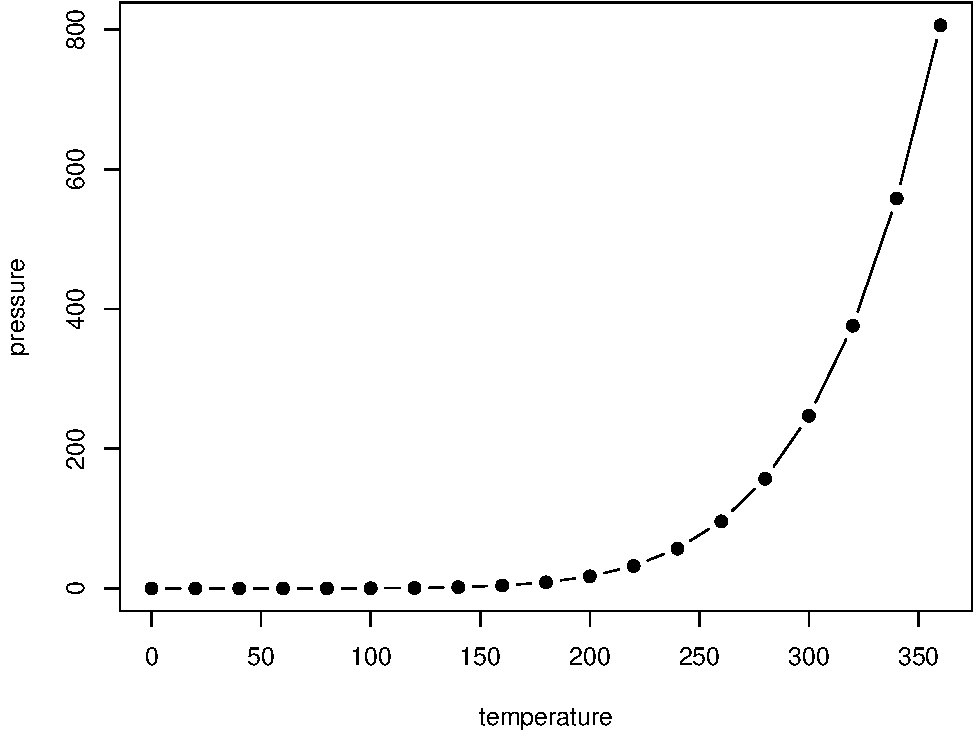
\includegraphics[width=0.8\linewidth,alt={Plot with connected points showing that vapor pressure of mercury increases exponentially as temperature increases.}]{02-cross-refs_files/figure-latex/nice-fig-1} 

}

\caption{Here is a nice figure!}\label{fig:nice-fig}
\end{figure}

Don't miss Table \ref{tab:nice-tab}.

\begin{Shaded}
\begin{Highlighting}[]
\NormalTok{knitr}\SpecialCharTok{::}\FunctionTok{kable}\NormalTok{(}
  \FunctionTok{head}\NormalTok{(pressure, }\DecValTok{10}\NormalTok{), }\AttributeTok{caption =} \StringTok{\textquotesingle{}Here is a nice table!\textquotesingle{}}\NormalTok{,}
  \AttributeTok{booktabs =} \ConstantTok{TRUE}
\NormalTok{)}
\end{Highlighting}
\end{Shaded}

\begin{table}

\caption{\label{tab:nice-tab}Here is a nice table!}
\centering
\begin{tabular}[t]{rr}
\toprule
temperature & pressure\\
\midrule
0 & 0.0002\\
20 & 0.0012\\
40 & 0.0060\\
60 & 0.0300\\
80 & 0.0900\\
\addlinespace
100 & 0.2700\\
120 & 0.7500\\
140 & 1.8500\\
160 & 4.2000\\
180 & 8.8000\\
\bottomrule
\end{tabular}
\end{table}

\chapter{Parts}\label{parts}

You can add parts to organize one or more book chapters together. Parts can be inserted at the top of an .Rmd file, before the first-level chapter heading in that same file.

Add a numbered part: \texttt{\#\ (PART)\ Act\ one\ \{-\}} (followed by \texttt{\#\ A\ chapter})

Add an unnumbered part: \texttt{\#\ (PART\textbackslash{}*)\ Act\ one\ \{-\}} (followed by \texttt{\#\ A\ chapter})

Add an appendix as a special kind of un-numbered part: \texttt{\#\ (APPENDIX)\ Other\ stuff\ \{-\}} (followed by \texttt{\#\ A\ chapter}). Chapters in an appendix are prepended with letters instead of numbers.

\chapter{Footnotes and citations}\label{footnotes-and-citations}

\section{Footnotes}\label{footnotes}

Footnotes are put inside the square brackets after a caret \texttt{\^{}{[}{]}}. Like this one \footnote{This is a footnote.}.

\section{Citations}\label{citations}

Reference items in your bibliography file(s) using \texttt{@key}.

For example, we are using the \textbf{bookdown} package \citep{R-bookdown} (check out the last code chunk in index.Rmd to see how this citation key was added) in this sample book, which was built on top of R Markdown and \textbf{knitr} \citep{xie2015} (this citation was added manually in an external file book.bib).
Note that the \texttt{.bib} files need to be listed in the index.Rmd with the YAML \texttt{bibliography} key.

The \texttt{bs4\_book} theme makes footnotes appear inline when you click on them. In this example book, we added \texttt{csl:\ chicago-fullnote-bibliography.csl} to the \texttt{index.Rmd} YAML, and include the \texttt{.csl} file. To download a new style, we recommend: \url{https://www.zotero.org/styles/}

The RStudio Visual Markdown Editor can also make it easier to insert citations: \url{https://rstudio.github.io/visual-markdown-editing/\#/citations}

\chapter{Blocks}\label{blocks}

\section{Equations}\label{equations}

Here is an equation.

\begin{equation} 
  f\left(k\right) = \binom{n}{k} p^k\left(1-p\right)^{n-k}
  \label{eq:binom}
\end{equation}

You may refer to using \texttt{\textbackslash{}@ref(eq:binom)}, like see Equation \eqref{eq:binom}.

\section{Theorems and proofs}\label{theorems-and-proofs}

Labeled theorems can be referenced in text using \texttt{\textbackslash{}@ref(thm:tri)}, for example, check out this smart theorem \ref{thm:tri}.

\begin{theorem}
\protect\hypertarget{thm:tri}{}\label{thm:tri}For a right triangle, if \(c\) denotes the \emph{length} of the hypotenuse
and \(a\) and \(b\) denote the lengths of the \textbf{other} two sides, we have
\[a^2 + b^2 = c^2\]
\end{theorem}

Read more here \url{https://bookdown.org/yihui/bookdown/markdown-extensions-by-bookdown.html}.

\section{Callout blocks}\label{callout-blocks}

The \texttt{bs4\_book} theme also includes special callout blocks, like this \texttt{.rmdnote}.

You can use \textbf{markdown} inside a block.

\begin{Shaded}
\begin{Highlighting}[]
\FunctionTok{head}\NormalTok{(beaver1, }\AttributeTok{n =} \DecValTok{5}\NormalTok{)}
\CommentTok{\#\textgreater{}   day time  temp activ}
\CommentTok{\#\textgreater{} 1 346  840 36.33     0}
\CommentTok{\#\textgreater{} 2 346  850 36.34     0}
\CommentTok{\#\textgreater{} 3 346  900 36.35     0}
\CommentTok{\#\textgreater{} 4 346  910 36.42     0}
\CommentTok{\#\textgreater{} 5 346  920 36.55     0}
\end{Highlighting}
\end{Shaded}

It is up to the user to define the appearance of these blocks for LaTeX output.

You may also use: \texttt{.rmdcaution}, \texttt{.rmdimportant}, \texttt{.rmdtip}, or \texttt{.rmdwarning} as the block name.

The R Markdown Cookbook provides more help on how to use custom blocks to design your own callouts: \url{https://bookdown.org/yihui/rmarkdown-cookbook/custom-blocks.html}

\chapter{Sharing your book}\label{sharing-your-book}

\section{Publishing}\label{publishing}

HTML books can be published online, see: \url{https://bookdown.org/yihui/bookdown/publishing.html}

\section{404 pages}\label{pages}

By default, users will be directed to a 404 page if they try to access a webpage that cannot be found. If you'd like to customize your 404 page instead of using the default, you may add either a \texttt{\_404.Rmd} or \texttt{\_404.md} file to your project root and use code and/or Markdown syntax.

\section{Metadata for sharing}\label{metadata-for-sharing}

Bookdown HTML books will provide HTML metadata for social sharing on platforms like Twitter, Facebook, and LinkedIn, using information you provide in the \texttt{index.Rmd} YAML. To setup, set the \texttt{url} for your book and the path to your \texttt{cover-image} file. Your book's \texttt{title} and \texttt{description} are also used.

This \texttt{bs4\_book} provides enhanced metadata for social sharing, so that each chapter shared will have a unique description, auto-generated based on the content.

Specify your book's source repository on GitHub as the \texttt{repo} in the \texttt{\_output.yml} file, which allows users to view each chapter's source file or suggest an edit. Read more about the features of this output format here:

\url{https://pkgs.rstudio.com/bookdown/reference/bs4_book.html}

Or use:

\begin{Shaded}
\begin{Highlighting}[]
\NormalTok{?bookdown}\SpecialCharTok{::}\NormalTok{bs4\_book}
\end{Highlighting}
\end{Shaded}


  \bibliography{book.bib,packages.bib}

\end{document}
